\documentclass[11pt,a4paper]{article}
\usepackage[spanish,es-tabla]{babel}
\usepackage[utf8]{inputenc}
\usepackage[T1]{fontenc}
\usepackage{lmodern}
\usepackage{amsmath,amssymb,mathtools}
\usepackage{geometry}
\usepackage{booktabs,longtable,array}
\usepackage{enumitem}
\usepackage{xcolor}
\usepackage{listings}
\geometry{margin=2.4cm}
\setlength{\parskip}{0.5em}
\setlength{\parindent}{0pt}

\lstdefinestyle{code}{
  basicstyle=\ttfamily\small,
  breaklines=true,
  columns=fullflexible,
  frame=single,
  backgroundcolor=\color{black!3}
}
\lstset{style=code,literate={≔}{{$\coloneqq$}}1 {≠}{{$\neq$}}1 {∅}{{$\emptyset$}}1 {ℕ}{{$\mathbb{N}$}}1 {ε}{{$\varepsilon$}}1}

\title{Práctica 4: WHILE y codificación\\\large Salma Boulagna Moreno}
\author{Teoría de Autómatas y Lenguajes Formales}
\date{\today}

\begin{document}
\maketitle

\section{Actividad 1: suma de tres valores en WHILE}
\begin{center}
    \centering
    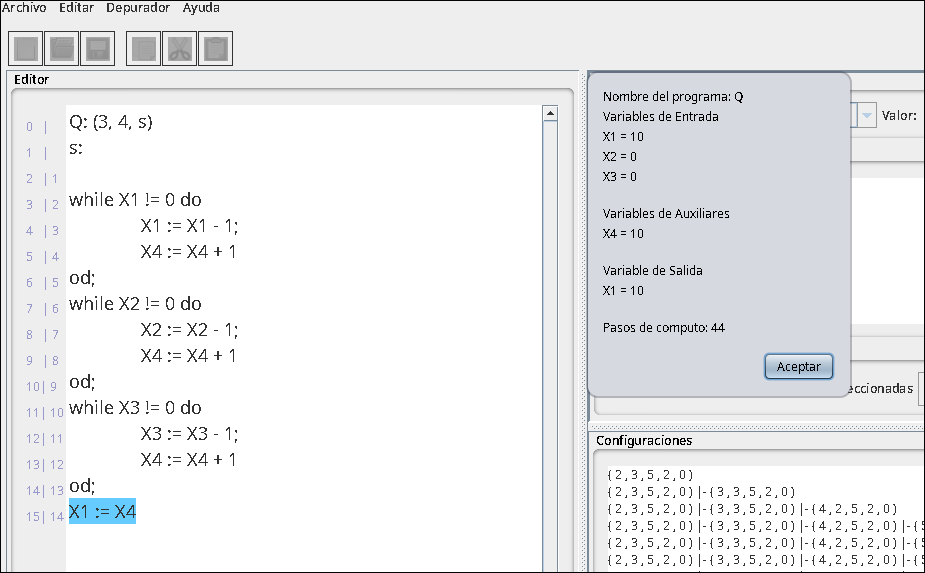
\includegraphics[width=0.75\linewidth]{Imagen pegada.png}
\end{center}
\subsection{Idea de diseño}
Se pide escribir un programa WHILE que calcule la suma de tres valores naturales. La función que se quiere obtener es:
\[
F_Q(x_1,x_2,x_3)=x_1+x_2+x_3.
\]

Para hacerlo se utiliza una variable auxiliar, $X_4$, como acumulador. La idea es recorrer las tres variables de entrada y, mientras cada una sea distinta de cero, restarle una unidad y sumar una unidad en $X_4$. Cuando los tres bucles han terminado, el valor acumulado se copia en $X_1$, ya que la función calculada por un programa WHILE se lee en la primera variable.

\subsection{Programa usado en Python}
El programa se ha escrito como una cadena para poder ejecutarlo con la librería \texttt{whilelanguage}:

\begin{lstlisting}[language=Python]
from python.whilelanguage import *
from python.whilelanguage.encoding import *

S = """(3,
while X1 != 0 do
    X1 := X1 - 1;
    X4 := X4 + 1
od;
while X2 != 0 do
    X2 := X2 - 1;
    X4 := X4 + 1
od;
while X3 != 0 do
    X3 := X3 - 1;
    X4 := X4 + 1
od;
X1 := X4)"""

print("tq", t_steps(S, [3, 5, 2]))
print("calq:", f_function(S, [3, 5, 2]))
\end{lstlisting}

\subsection{Ejecución y resultado}
La entrada comprobada es $(3,5,2)$, por lo que el valor esperado es:
\[
3+5+2=10.
\]

La ejecución devuelve:

\begin{lstlisting}
tq 44
calq: 10
\end{lstlisting}

Por tanto:
\[
F_Q(3,5,2)=10,
\qquad
T_Q(3,5,2)=44.
\]

El resultado final coincide con la suma esperada. Además, el valor de \texttt{t\_steps} indica que el programa tarda $44$ pasos en alcanzar la configuración final para esa entrada.

\section{Actividad 2: programa que calcula la función diverge}

\subsection{Definición del programa}
La función \texttt{diverge} es una función sin argumentos que no termina nunca. Como las variables del programa empiezan inicializadas a cero, basta con hacer que $X_1$ valga uno y después entrar en un bucle que nunca pueda finalizar.

El código WHILE elegido es:

\begin{lstlisting}
X1:=X1+1; while X1!=0 do X1:=X1+1 od
\end{lstlisting}

En Python se guarda en la variable \texttt{D}:

\begin{lstlisting}[language=Python]
D = "X1:=X1+1; while X1!=0 do X1:=X1+1 od"
\end{lstlisting}

\subsection{Justificación}
Al comenzar la ejecución se tiene:
\[
X_1=0.
\]

La primera instrucción hace que:
\[
X_1=1.
\]

A partir de ahí se evalúa el bucle:

\begin{lstlisting}
while X1!=0 do X1:=X1+1 od
\end{lstlisting}

Como dentro del bucle $X_1$ aumenta en una unidad, nunca vuelve a valer cero. Por tanto, la condición $X_1\neq 0$ sigue siendo verdadera indefinidamente y el programa no se detiene.

\subsection{Codificación}
La función \texttt{while2n} utilizada en la práctica recibe dos argumentos: el número de variables de entrada y el código del programa. Como \texttt{diverge} tiene cero argumentos, se codifica con:

\begin{lstlisting}[language=Python]
print(while2n(0, D))
\end{lstlisting}

La salida obtenida es:

\begin{lstlisting}
139273919255627
\end{lstlisting}

Así, la codificación del programa completo es:
\[
\ulcorner (0,D) \urcorner = 139273919255627.
\]

Si únicamente se codifican las instrucciones, sin añadir el número de variables de entrada, se obtiene con \texttt{code2n(D)}. En este caso:

\begin{lstlisting}
code2n(D) = 16689751
\end{lstlisting}

\section{Actividad 3: enumeración de vectores de $\mathbb{N}^{*}$}

\subsection{Idea de diseño}
El conjunto $\mathbb{N}^{*}$ contiene todos los vectores finitos de naturales:
\[
\mathbb{N}^{*}=\bigcup_{n\geq 0}\mathbb{N}^{n}.
\]

En particular, contiene el vector vacío, vectores de longitud uno, vectores de longitud dos, etc. Para enumerarlos se utiliza la decodificación de Gödel implementada en la librería. La idea es recorrer los números naturales y aplicar \texttt{godeldecoding} a cada uno de ellos.

\subsection{Función implementada}
\begin{lstlisting}[language=Python]
def primeros_vectores(k):
    salida = []

    for numero in range(k):
        salida.append(godeldecoding(numero))

    return salida

print(primeros_vectores(10))
\end{lstlisting}

\subsection{Comprobación para $k=10$}
La ejecución para los diez primeros vectores produce:

\begin{lstlisting}
[[], [0], [0, 0], [1], [0, 0, 0], [1, 0], [2],
 [0, 0, 0, 0], [1, 0, 0], [0, 1]]
\end{lstlisting}

\subsection{Interpretación}
La función recorre:
\[
0,1,2,3,\ldots,k-1
\]
y decodifica cada número natural como un vector finito. Por eso, el orden de aparición de los vectores es el orden inducido por la codificación de Gödel usada por la librería.

Esto muestra que $\mathbb{N}^{*}$ es enumerable: existe un procedimiento efectivo que permite listar todos sus elementos.

\section{Actividad 4: enumeración de programas WHILE}

\subsection{Idea de diseño}
Los programas WHILE también se pueden codificar mediante números naturales. Por tanto, para enumerar programas basta con recorrer números naturales y decodificar cada uno con la función \texttt{n2while} de la librería.

\subsection{Función implementada}
\begin{lstlisting}[language=Python]
def primeros_while(k):
    listado = []

    for codigo in range(k):
        listado.append(n2while(codigo))

    return listado

lista = primeros_while(10)

for posicion, programa in enumerate(lista):
    print(posicion, programa)
\end{lstlisting}

\subsection{Comprobación para $k=10$}
La salida obtenida es:

\begin{lstlisting}
0 (0, X1≔0)
1 (1, X1≔0)
2 (0, X1≔0; X1≔0)
3 (2, X1≔0)
4 (1, X1≔0; X1≔0)
5 (0, X1≔X1)
6 (3, X1≔0)
7 (2, X1≔0; X1≔0)
8 (1, X1≔X1)
9 (0, X1≔0; X1≔0; X1≔0)
\end{lstlisting}

\subsection{Interpretación}
Cada número natural se interpreta como la codificación de un programa WHILE. La función \texttt{n2while} realiza la decodificación y devuelve el programa correspondiente.

El procedimiento seguido es:
\[
0\mapsto n2while(0),\quad
1\mapsto n2while(1),\quad
2\mapsto n2while(2),\quad \ldots
\]

Por tanto, los programas WHILE forman un conjunto enumerable. Esta idea es importante porque permite tratar los programas como datos y asignar a cada programa un número natural.


\section{Conclusión}

En esta práctica se ha trabajado con programas WHILE, funciones parciales y codificaciones mediante números naturales. Primero se ha implementado un programa que calcula la suma de tres valores y se ha comprobado tanto su resultado como su tiempo de parada. Después se ha construido un programa que no termina, representando así la función \texttt{diverge}.

También se ha utilizado la librería de codificación para enumerar tanto los vectores de $\mathbb{N}^{*}$ como los programas WHILE. En ambos casos se usa la misma idea teórica: recorrer los números naturales y decodificar cada número según la codificación correspondiente.

\end{document}
